
% Honours Report Template
% updated May 2013
%
\documentclass[a4paper,12pt]{article}
%\makeatletter
%\renewcommand\paragraph{\@startsection{paragraph}{4}{\z@}%
%{-2.5ex\@plus -1ex \@minus -.25ex}%
%{1.25ex \@plus .25ex}%
%{\normalfont\normalsize\bfseries}}
%\makeatother
%\setcounter{secnumdepth}{4} % how many sectioning levels to assign numbers to
%\setcounter{tocdepth}{4}    % how many sectioning levels to show in ToC
%
\usepackage{pbox}
\usepackage{epsfig}
\usepackage{latexsym}
\usepackage{graphicx}
\usepackage[square,numbers]{./natbib/natbib}
\usepackage{url}
\usepackage{graphicx}
% It also sets the bibliographystyle to plainnat; for more information on
% natbib citation styles, see the natbib documentation, a copy of which
% is archived at http://www.jmlr.org/format/natbib.pdf
\usepackage{setspace}
\usepackage{amsmath}
\usepackage{amssymb}
\usepackage{amsfonts}
\usepackage{color}

%\graphicspath{{./figures/}
%Formatting-------------------------------------------------------------------
%\renewcommand{\refname}{\textbf{Literature}}
%
\renewcommand{\contentsname}{\small\textbf{{\center Table of Contents}}}
%
\setlength{\textheight}{8.8in}
%
\setlength{\topmargin}{-1.5cm}
%
\doublespacing
%\setlength{\textwidth}{17cm}
%
%\setlength{\oddsidemargin}{-0.1714in}
%
% Boxit -----------------------------------------------------------
\setlength{\fboxrule}{0.2mm} \setlength{\fboxsep}{4mm}
%
\newsavebox{\savepar}
\newenvironment{boxit}{\begin{lrbox}{\savepar}
        \begin{minipage}[b]{4.6in}}
        {\end{minipage}\end{lrbox}\fbox{\usebox{\savepar}}}
        
        
 \hyphenation{op-tical net-works Mathe-ma-tical street-scape street-scapes aes-the-tics aes-the-tic com-pu-ting geo-metric Geo-me-tric geo-metry boun-da-ries de-ve-lop-ment know-ledge mani-fold mani-folds high-di-men-sio-nal}
%
%
%
% Document-----------------------------------------------------------------------
%
\begin{document}
%
\title{\bf Technology \& User Engagement}
%
\author{Ross Bille\\
School of Electrical Engineering \& Computer Science\\
The University of Newcastle\\ Callaghan NSW 2308, Australia\\
Email: \texttt{c3127333@uon.edu.au} } 
\maketitle


\newpage
\begin{abstract}%
\noindent Document abstract 
\end{abstract}

\pagebreak

\tableofcontents

\pagebreak

\listoffigures        

\pagebreak

\section{Introduction}

%User engagement and why we need it
%introduction to city evolutions project

\section{Current Fields Utilising Technology for User Engagement}
%where these methods can take effect
The following sections 
\subsection{Workplace}
\subsection{Education}
\subsection{Therapy}
\subsection{Community}


\section{Techniques to Enhance User Engagement}

\subsection{The Skinner Box}
The Skinner Box is a technique named by B.F. Skinner describing a small cage which houses a small animal, a lever and a way of delivering rewards to the animal~\citep{openingSkinersBox}. The idea was to train the animal to continuously hit the lever. The animal gets rewarded at random intervals for lever pressing, with the possibility of punishment if the lever is not pressed (usually by electric shock). This technique has been around since the 1930’s and has been implemented in video games since their inception~\citep{theSkinnerBox}.
\\
Game designers have expanded the Skinner Box concept and made it feel like second nature to players. They have done this by offering virtual rewards to players who achieve pre-defined goals (this is obvious in any games that have levels and/or virtual currency) and recently by punishing players for not playing regularly (usually by devaluing the players hard earned virtual currency or by making in-game possessions deteriorate).
\\
The Skinner Box concept is a great way to develop players’ obsession to a game while offering no real world reward, often leaving the player wondering why they wasted so much time on the game~\citep{fiveCreepyWays} 

\subsection{Gamification}
Gamification is the process of integrating game dynamics and techniques into non-game processes. This is usually done to increase interaction, productivity or satisfaction.
\subsubsection{The History of Gamification}
\subsubsection{Elements in Game Design}
Gamification takes advantage of various features that are present in game design. The following paragraphs discuss the effectiveness of these features as well as the importance of their potential applications in enhancing user interactions beyond the gaming culture. 
\paragraph{\indent~Rewards}
\paragraph{\indent~Competition}
\paragraph{\indent~Stories}

\subsection{Virtual Reality}
\subsection{Effort Reduction}
\subsection{Usability}
\subsection{Social Media}
\subsection{Education}
%closing the loop etc
%
\section{City Evolutions}
\subsection{Analysis}
\section{Results}
\begin{figure}[ht!]
	\centering
	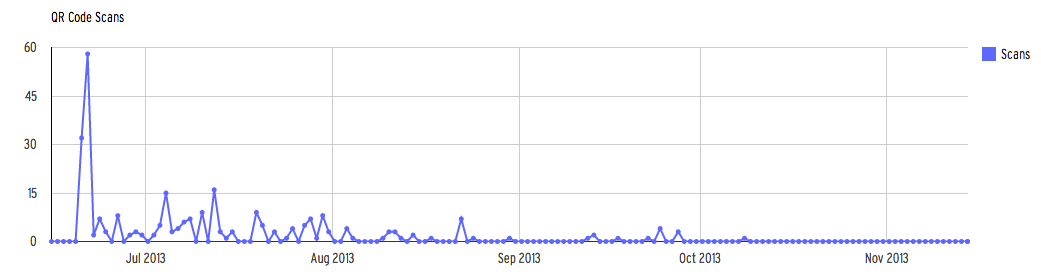
\includegraphics[width=150mm]{./images/OverallQRCodeDownload}
	\caption{QR Code - Overall scans}
	\label{QR-overall-access-overTime}
\end{figure}

\begin{figure}[ht!]
	\centering
	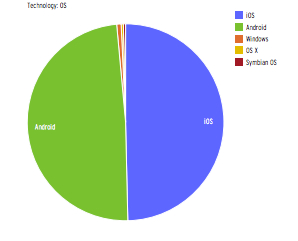
\includegraphics[width=50mm]{./images/OSAccess}
	\caption{QR Code - OS spread}
	\label{QR-OS-access}
\end{figure}

\begin{figure}[ht!]
	\centering
	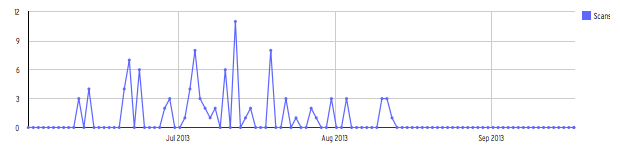
\includegraphics[width=150mm]{./images/threkeld-scans}
	\caption{QR Code - Threlkeld Speak scans}
	\label{QR-threkeld}
\end{figure}

\begin{figure}[ht!]
	\centering
	
\includegraphics[width=75mm]{./images/qrcode-threlkeld}
	\caption{QR Code - Threlkeld Speak}
	\label{QR-threkeld-barcode}
\end{figure}

\begin{table}
	\centering
	\begin{tabular}{|c|c|c|}\hline
		\textbf{Application} & 	\textbf{Number of Scans} & \textbf{Interactivity (see table~\ref{table:interactivity-description})} \\\hline
		Macquaries Chest & 2 & Low\\
		Car Culture & 3 & None\\
		Lansescape & 34 & Medium\\
		Coal Collector & 30 & \\
		Place of Coal & 6 & \\
		Dreaming & 3 & \\
		Settling In & 28 & \\
		Major Morisset & 36 & \\
		Evolutions & 6 & \\
		Shanghai & 2 & \\
		Boom \& Bust & 2 & \\
		Threlkeld 	&	132 & \\\hline
	\end{tabular}
	\caption{City Evolutions Applications and their popularity}
	\label{table:application-popularity}
\end{table}

\begin{table}
	\centering
	\bgroup
	\def\arraystretch{2.5}%  1 is the default, change whatever you need
	\begin{tabular}{|l|l|}\hline
		\textbf{Level} 	& \textbf{Description}\\\hline
		None 	& \pbox{20cm}{No user input is taken at all} \\\hline
		Low 	& \pbox{20cm}{Generally a single has basic control over the application\\ 
				  			  i.e. User makes movement to trigger the application to take action.} \\\hline
		Medium 	& \pbox{20cm}{Users have basic control over the application and are given constant\\
							  feedback, the more users the more feedback is received.}\\\hline
		High 	& \pbox{20cm}{Users have fine grained control over the application,\\ 
							  with constant feedback and a reason to come back to the application\\
							  i.e. scores are saved, competitions are run, etc.}\\\hline
	\end{tabular}
	\egroup
	\caption{Description of interactivity levels used in \ref{table:application-popularity}}
	\label{table:interactivity-description}
\end{table}


\section{Discussion}
%
Give an extended and detailed discussion of your study. Explain what we can learn from your study.
%

\section{Conclusion}
%
A brief final summary of the main achievements and outcomes. Possibly some suggestions for future work that can follow on from your project.%

\section{Glossary}
%
\subsection*{Acknowledgements}
The author is grateful to ....
%
\vskip 0.2in
\newpage
\bibliographystyle{apalike}
\bibliography{./literature.bib}

\end{document}
